\section{Theorie}
\label{sec:Theorie}
Im ursprünglichen Stern-Gerlach Versuch ist die Aufspaltung eines Silber-Atomstrahls beim
Durchlauf eines inhomogenen Magnetfeldes zu beobachten.
An den Spin vom äußeren Elektron des Silber-Atoms koppelt ein magnetisches
Moment $\mu$, welches für die Ablenkung verantwortlich ist.
Das Magnetische Moment setzt sich aus dem Eigendrehimpuls $S$,
dem Bahndrehimpuls $L$ und dem Kernspin $I$ zusammen zu: $\mu=\mu_\mathrm{S}+\mu_\mathrm{L}+\mu_\mathrm{I}$.
Hierbei ist $\mu_\mathrm{I}$ vernachlässigbar klein gegenüber den anderen
magnetischen Momenten.
Bei Atomen mit einem Valenzelektron in der s-Schale ist der Bahndrehimpuls
$L$ gleich null und somit auch $\mu_\mathrm{L}$.
Es bleibt ein magnetisches Moment von:
\begin{align}
  \vec{\mu}_\mathrm{S}=-\frac{e}{2m}g_\mathrm{S}\vec{S}
\end{align}
übrig. Das gyromagnetische Verhältnis wird mit $g_\mathrm{S}\approx 2$ bezeichnet.
Besteht ein Magnetfeld in z-Richtung, so sind zwei Spineinstellungen möglich und
es gilt für die z-Komponente des magnetischen Momentes:
\begin{align}
  \mu_\mathrm{s_\mathrm{z}}=-g_\mathrm{s}m_\mathrm{s}\mu_\mathrm{B}
\end{align}
mit $\mu_\mathrm{B}=\frac{e}{2m}\hbar$ dem bohrschen Magneton.
Bei der Wechselwirkung der Atomen mit einem inhomogenen Magnetfeld
in z-Richtung wirkt auf diese eine Kraft:
\begin{align}
  F_\mathrm{z}=-m\mu_\mathrm{B}\frac{\partial B}{\partial z}
\end{align}
in z-Richtung. Hier beschreibt $m$ die Eigenwerte von $\mu_\mathrm{S}$.

\subsection{Beschreibung der Versuchsapparatur}
In diesem Versuch wird zur Untersuchung der Richtungsquantelung Kalium genutzt.
Das Kalium wird in einem Ofen verdampft und mittels Blenden zu einem Strahl gebündelt.
Sowohl die Teilchendichte $\rho(v)$ als auch die Geschwindigkeit $v$ der Atome im Teilchenstrahl
hängen von der Ofentemperatur $T$ ab. Im Ofen folgen die Atome einer
maxwellschen Geschwindigkeitsverteilung:
\begin{align}
  \rho(v)dv=\frac{4}{\sqrt{\pi}\alpha^3}v^2 \exp{\frac{-v^2}{\alpha^3}}dv
\end{align}
mit $\alpha=\sqrt{\frac{2kT}{m}}$.\\
Für den messbaren Teilchenstrom $I(v)=\rho(v)v$ gilt damit:
\begin{align}
 I(v)=\frac{4}{\sqrt{\pi}\alpha^3}v^3 \exp{\frac{-v^2}{\alpha^3}}\label{eqn:teilchenstrom},
\end{align}
mit einem Maximum bei $v_\mathrm{m}=\sqrt{\frac{3}{2}\alpha}$.
Bei einem senkrechten Eintritt in ein Magnetfeld mit beinahe konstantem Gradienten folgen
die Atome einer parabelförmigen Flugbahn. Die Ablenkung ist dabei umgekehrt proportional
zum Geschwindigkeitsquadrat der Atome.
Beobachtbar ist diese Ablenkung bei einem Feldgradienten
in Größenordnung des Strahlendurchmessers.
Der in diesem Versuch genutzte Elektromagnet besitzt ein zylinderförmiges
Polschuhprofil, gezeigt in Abbildung \ref{fig:magnet}.
\begin{figure}
   \centering
    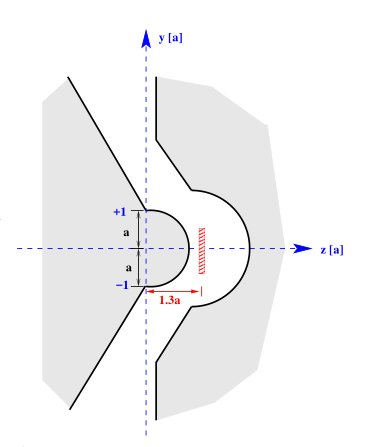
\includegraphics[width=0.5\textwidth]{magnet.PNG}
    \caption{Querschnitt des genutzten Magneten. Rot markiert ist der Bereich mit konstantem Feldgradienten.\cite{skript}}
    \label{fig:magnet}
    \FloatBarrier
\end{figure}
Dessen Magnetfeld entspricht dem zweier stromdurchflossener Drähte im Abstand $2a$
mit entgegengesetzter Stromrichtung.
Ist der Atomstrahl circa $1,3a$ von den gedachten Drähten entfernt, so ist
der Feldgradient in y-Richtung beinahe unabhängig von y.
Für den Feldgradienten gilt dann:
\begin{align}
  \frac{\partial B}{\partial z}=0,968\frac{B}{a}\label{eqn:grad}
\end{align}
mit $B=\mu_\mathrm{0}\mu_\mathrm{r}\frac{I}{\pi}\frac{a}{r^2}$ dem magnetischen
Feld an der Stelle r des Zweidratkonstrukts.
In einem Langmuir-Taylor Detektor werden die Teilchen detektiert.
Der LT-Detektor setzt sich zusammen aus einem beheizten Wolfram Draht, umgeben
von einem Nickelzylinder. Zwischen den Elementen liegt eine Abzugsspannung an.
Das Kalium wird an der Oberfläche des Wolframs
ionisiert und als Ionen emittiert. Die Ionisierungsenergie der Kaliumatome
muss hier geringer sein als die Austrittsarbeit des Wolframs.
Über die Flugbahn des Atomstrahls lässt sich die Intensitätsverteilung
bestimmen. Ohne ein Magnetfeld lässt sich die Nullposition mit nur einem
Maximum messen. Mit eingeschaltetem Magnetfeld formen sich zwei Intensitätsmaxima
rechts und links der Nullposition aus.
Für den Abstand zwischen Nullposition und jeweiligem Maximum gilt:
\begin{align}
 s=\mu_\mathrm{sz}\frac{l\cdot L\left(1-\frac{L}{2l}\right)}{6kT}\cdot\frac{\partial B}{\partial z} \label{eqn:abstand}
\end{align}
mit $L$ der Länge der Polschuhe und $l$ dem Abstand zwischen
der Eintrittsblende $B_\mathrm{4}$, zu sehen in Abbildung \ref{fig:schema} und Wolframdraht.
\begin{figure}
   \centering
    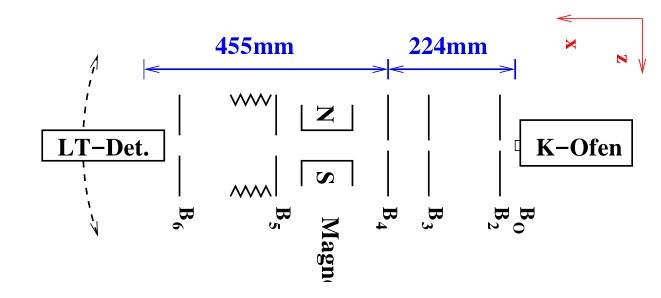
\includegraphics[width=0.5\textwidth]{schema.PNG}
    \caption{Die Position der Eintrittsblende.\cite{skript}}
    \label{fig:schema}
    \FloatBarrier
\end{figure}
